\documentclass[conference]{IEEEtran}
\usepackage{amsmath,amssymb,booktabs,graphicx,url}
\usepackage[hidelinks]{hyperref}
\usepackage{tikz}
\usetikzlibrary{arrows.meta,positioning}
\graphicspath{{../figures/}}
\title{Cross-Institution Reliability of Temporal Attributions in Network Traffic Forecasting}
\author{\IEEEauthorblockN{Anonymous research draft}\IEEEauthorblockA{Author information and conference formatting to be completed before submission}}
\begin{document}\maketitle
\begin{abstract}
A traffic forecaster can transfer to a new institution without establishing that its temporal explanations remain useful. We examine this distinction using a frozen protocol on 48 institutions from CESNET-TimeSeries26: 32 for source training, eight for validation, and eight unseen targets. Ridge, DLinear, and gated recurrent forecasters predict hourly traffic at one- and six-hour endpoints from one week of history. We separate forecast error, numerical attribution checks, and ranking alignment under two controlled history replacements. Exact seven-group Shapley allocations, occlusion, recency, and numerically screened integrated gradients are evaluated with two attribution references. The prespecified primary contrast is target-minus-source Shapley ranking alignment for the frozen one-hour GRU. Across seven complete matched pairs, the difference is $-0.0189$ with a nominal paired block-bootstrap 95\% interval of $[-0.0891,0.0533]$. This does not establish either systematic degradation or equivalence. Ridge, DLinear, and GRU achieve similar one-hour target MASE (0.681, 0.682, and 0.684), whereas 210 of 3,360 integrated-gradient cases fail the fixed numerical acceptance checks. These findings support an auditable, reference-explicit evaluation of attribution transfer; they do not establish a universally superior explainer or cross-network causal reliability.
\end{abstract}
\begin{IEEEkeywords}network traffic forecasting, explainability, institution transfer, temporal attribution, evaluation\end{IEEEkeywords}

\section{Introduction}
Network traffic forecasting supports resource planning, but a forecast and an explanation answer different operational questions. Forecast error measures agreement with subsequent observations. A temporal attribution distributes a prediction contrast over historical inputs. A ranking test measures how an ordering responds to a specified intervention on those inputs. Success on one does not certify the others. This distinction becomes consequential when a pooled forecaster is deployed to an institution absent from model fitting.

Transferable traffic prediction is established research: TransMUSE studies transfer across edge cohorts~\cite{transmuse}. Network forecasting explanations and their operational use are also established, including AIChronoLens~\cite{aichrono}. More recent work studies explanation generalization for time series~\cite{timesae}. Accordingly, the question here is narrower than whether transfer or explainable forecasting is possible: under a fixed, institution-disjoint network deployment protocol, what evidence supports the reliability of temporal attribution rankings, and how does that evidence depend on the attribution contrast and measurement operator?

We use a public multi-year traffic dataset~\cite{cesnet26,dataset}. We retain source-only fitting, unseen validation institutions, fixed target institutions, timestamp-matched explanation cases, repeated neural seeds, and a prespecified primary comparison. Our contribution is an empirical audit design and its executed evidence, rather than a new attribution algorithm. Specifically, we provide (i) a reproducible institution-disjoint benchmark with explicit missingness and effective sample counts; (ii) separate checks of numerical attribution behavior and controlled-operator ranking alignment; and (iii) a paired transfer estimate with reference, horizon, model, and bias-calibration analyses clearly designated as secondary.

The primary result is inconclusive about systematic ranking degradation. We retain it despite stronger nominal secondary contrasts under a different attribution reference; those remain exploratory.

\section{Related Work and Scope}
\subsection{Forecasting and network explanations}
TransMUSE~\cite{transmuse} addresses service-aware model transfer and prediction performance. DLinear~\cite{dlinear} demonstrates the importance of simple linear forecasting baselines, motivating their inclusion alongside a GRU~\cite{gru}. CESNET's comparative forecasting work~\cite{comparison} and the CESNET-TimeSeries26 descriptor~\cite{cesnet26} motivate evaluation across institutions and time. Our compact model set is a controlled benchmark, not an exhaustive assessment of current forecasting architectures.

AIChronoLens~\cite{aichrono} relates explanations to temporal properties and forecast errors in mobile networks. Explanations of aggregated network predictors have also been studied~\cite{aggregated}, as have attacks on explainability in networking~\cite{deexp}. The present study does not introduce temporal explanation, aggregation analysis, error repair, or adversarial robustness. Its focus is a fixed source-to-unseen-institution comparison on institutional byte-volume series.

\subsection{Attribution semantics and evaluation}
Integrated gradients (IG) explains a path-dependent prediction contrast~\cite{ig}; Shapley attribution allocates a coalition game~\cite{shap}. Baseline choice changes the question being answered~\cite{manyshap,baselines}. Different nonlinear allocations therefore need not agree, and an efficiency identity alone cannot establish the substantive correctness of an explanation. Sanity checks~\cite{sanity}, learned perturbations~\cite{perturb}, and InterpretTime~\cite{interprettime} further motivate examining the evaluation procedure itself.

TIMING~\cite{timing} discusses opposing signed effects, temporal paths, and cumulative response metrics. We use a cumulative absolute sequential response, with an explicitly defined normalization; cancellation awareness is not claimed as new. TimeSAE~\cite{timesae}, accepted at ICML 2026, already examines explanation generalization under shift. Our study differs in deployment unit, observed institutional traffic, input-day groups, and a numerical-versus-ranking audit. We do not implement or claim to outperform TimeSAE, TIMING, or other specialized explainers. The novelty claim is thus a bounded combination of experimental controls and empirical evidence in this network setting, subject to further venue-specific literature review.

\section{Data and Frozen Deployment Protocol}
\subsection{Provenance and eligibility}
We use the official hourly institutional \texttt{n\_bytes} files from CESNET-TimeSeries26, Zenodo record 21945629, under CC BY 4.0~\cite{dataset}. The dataset covers institutions within the CESNET3 network~\cite{cesnet26}; institutions are not independent ISPs. We verified the downloaded archive checksum, source-member SHA-256 values, and hashes of all 48 derived files. Traffic units are decimal GB ($10^9$ bytes). No attack-detection labels or synthetic traffic mixtures enter this benchmark.

Native time mappings identify hourly coverage. A usable hour has six native ten-minute records and an observed finite nonnegative value. We require all 168 historical hours and both forecast endpoints to be usable. We retain observed zeros, do not impute labels, and do not convert absent values into zeros. A conservative global flag excludes windows crossing 21 May--4 June 2024 because of a documented probe-artifact concern; its institution-specific scope is uncertain. This screening choice is not evidence that every institution was affected.

Twelve institutions used in earlier development are excluded from this study's membership. Among the remaining eligible institutions, four 2024 median-volume strata and deterministic SHA-256 ordering select 48 institutions: 32 source, eight validation, and eight target. Selection uses saved 2024 coverage and volume metadata, not final forecasting or attribution results. Eight one-to-one source--target pairs are matched within volume strata using 2024 median volume and coefficient of variation. These descriptors do not remove all institutional differences; matching is descriptive rather than a causal identification strategy.

\subsection{Chronology and observed sample}
Source training targets occur in 2024. Hyperparameters use the eight validation institutions during January--March 2025. Final target endpoints lie in the UTC intervals [8 April, 1 July) in 2025 and 2026, with forecast origins at hours divisible by six. The source and target explanation origins are intersected per pair and year, then up to 16 evenly spaced eligible origins are chosen without observing errors or explanation scores. IG uses four evenly spaced origins from that selection.

The resulting selection contains 480 institution-origin cases per fitted model, rather than the planned maximum 512. Pair 2 (source 160, target 192) has no common eligible origins in 2026; its 2025 cases remain in descriptive outputs, while the two-year primary estimate uses seven complete pairs. Target forecasting has 15 available institution-year cells. In 2026, selected target institutions have only 50 or 129 eligible origins per available cell, versus 206 or 307 in 2025. These unequal counts arise from observed availability and the complete-history rule, not outcome-based pruning. Results describe eligible observations, not uninterrupted coverage of either calendar interval.

\begin{figure}[t]\centering
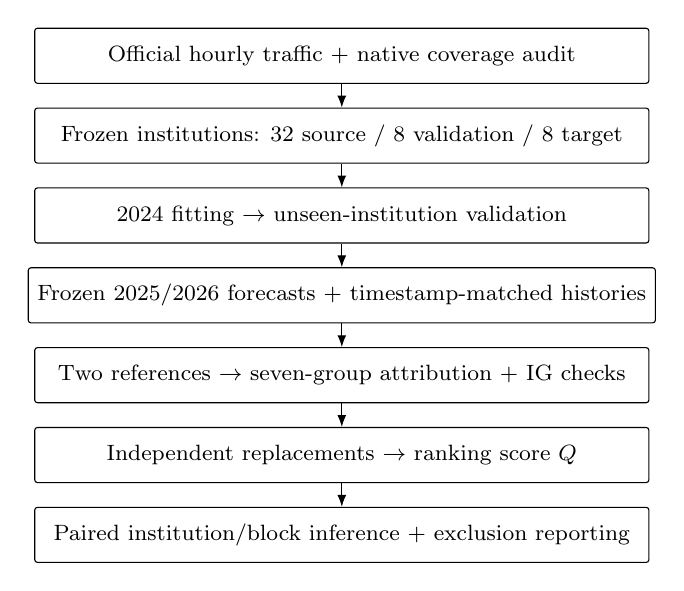
\begin{tikzpicture}[node distance=3mm, every node/.style={font=\footnotesize,align=center}, box/.style={draw,rounded corners=1pt,minimum width=7.8cm,minimum height=7mm},arr/.style={-{Latex[length=1.5mm]}}]
\node[box] (a) {Official hourly traffic + native coverage audit};
\node[box,below=of a] (b) {Frozen institutions: 32 source / 8 validation / 8 target};
\node[box,below=of b] (c) {2024 fitting $\rightarrow$ unseen-institution validation};
\node[box,below=of c] (d) {Frozen 2025/2026 forecasts + timestamp-matched histories};
\node[box,below=of d] (e) {Two references $\rightarrow$ seven-group attribution + IG checks};
\node[box,below=of e] (f) {Independent replacements $\rightarrow$ ranking score $Q$};
\node[box,below=of f] (g) {Paired institution/block inference + exclusion reporting};
\foreach \x/\y in {a/b,b/c,c/d,d/e,e/f,f/g}\draw[arr] (\x)--(\y);
\end{tikzpicture}
\caption{Executed pipeline. Target outcomes are opened only after the full protocol, code, membership, and analysis rules are hashed. Hashing is a local audit trail, not an external preregistration.}\label{fig:pipeline}
\end{figure}

\subsection{Predictors and fitting}
Inputs are 168 hourly GB values transformed by $\log(1+x)$. Models predict endpoints $h\in\{1,6\}$ directly, not the six intermediate hours. The deployed output is
\begin{equation}
F_h(x)=\exp\!\left(\max\{0,z_h(\log(1+x))\}\right)-1.
\end{equation}
All attributions include this transformation, clipping, and any source-trained normalization. A ridge model fits separate horizon heads with $\alpha\in\{0.1,1,10,100\}$; validation selects $0.1$ for both. DLinear has a 25-hour moving-average decomposition and two linear 168-to-2 maps. The GRU uses one layer with 32 hidden units and a correction to the last log input. The implementation and initializations are included with the checkpoints.

Neural training uses source-only scalar log-input mean and standard deviation, Adam, batch size 256, log-space MSE, gradient clipping at 1, and 1,024 sampled windows per source institution per epoch. A maximum of 30 epochs and patience five control stopping. Validation selects between learning rates $10^{-3}$ and $3\cdot10^{-4}$ using seed 42; seeds 123 and 2026 reuse the chosen setting. Selected rates are $3\cdot10^{-4}$ for DLinear and $10^{-3}$ for GRU. There are 227,478 eligible source windows and zero target institutions in gradient fitting. Training took approximately 318 seconds on a four-thread CPU run, excluding extraction and evaluation. Persistence, daily, and weekly seasonal forecasts supply additional baselines.

A secondary calibrated arm adds a per-institution, per-year, per-horizon median log residual from eligible 1--8 April observations. At least 24 examples are required; otherwise the offset is zero and flagged. Both source and target arms receive this treatment. This is bias calibration using local observations, not zero-shot transfer or neural fine-tuning. The frozen arm remains primary.

\section{Attribution and Ranking Measurements}
\subsection{Explicit explanation contrasts}
We partition each history into seven consecutive 24-hour groups, oldest to newest. The source-calendar reference is a source-training-only pooled median profile by hour of week. The history-hour-median reference repeats the input history's median for each hour of day across the week. Neither reference is fitted to future endpoints. They encode different contrast questions; disagreement does not itself indicate failure.

For each reference $r$ and observed input $x$, define a retained-group game $v(S)=F(x_S,r_{\bar S})$. We enumerate all $2^7=128$ coalitions and compute exact group Shapley values
\begin{equation}
\phi_j=\sum_{S\subseteq N\setminus\{j\}}\frac{|S|!(6-|S|)!}{7!}\big[v(S\cup\{j\})-v(S)\big].
\end{equation}
The sum is checked against $F(x)-F(r)$ in double precision. Occlusion ranks the absolute change after replacing one group; recency ranks newest groups first. Shapley and IG rank the absolute signed group sum. Consequently, opposing effects within a day can cancel in that day's attribution. This grouping choice limits interpretation below the daily scale.

IG integrates raw-GB gradients along the straight path from $r$ to $x$~\cite{ig}. Gauss--Legendre node counts are 32, 64, 128, 256, and 512. A case is accepted only when both completeness error and successive L1 attribution change satisfy fixed absolute-plus-relative tolerances: $10^{-8}$ GB plus $10^{-3}$ times the absolute prediction contrast or L1 attribution, respectively. Failed cases remain in the numerical audit and receive no IG ranking score. Numerical acceptance is not a proof that a path is on-manifold or that its ranking is useful.

\subsection{Controlled replacement tests}
The ranking test uses templates distinct from the attribution references. Within-day interpolation replaces a selected day by a straight line between that day's observed endpoints. It suppresses internal variation while preserving endpoint information, and is therefore not full feature deletion. Rotation replaces selected day blocks by their counterparts in a cyclic one-day shift of the observed week. This uses no future label but can still create unusual histories. We record the RMS log-input displacement of each template. Neither operator is asserted to sample natural counterfactual network traffic.

For an ordering $\pi$, replace its first $k$ groups sequentially, yielding $x^{(0)},\ldots,x^{(k)}$. Define
\begin{align}
C_k(\pi)&=\sum_{j=1}^{k}|F(x^{(j)})-F(x^{(j-1)})|,\\
U(\pi)&=\tfrac13\big(C_1(\pi)+C_2(\pi)+C_4(\pi)\big).
\end{align}
This cumulative absolute response is related to cancellation-aware evaluation~\cite{timing}. We enumerate all $7!=5,040$ rankings. Their exact mean utility $R$ is the random-order comparator; their maximum $O$ is a response-oracle upper bound. The reported alignment score is
\begin{equation}
Q(\pi)=\frac{U(\pi)-R}{O-R}.
\end{equation}
We mark $Q$ undefined when $O-R\leq10^{-9}$ GB. Otherwise $Q=0$ equals the random-order mean, $Q=1$ attains the operator-specific response oracle, and negative values are allowed. The oracle optimizes forecast response, not future forecast accuracy. Thus $Q$ is neither a probability, a causal demand score, nor a universal test of attribution correctness. Large changes can reflect brittleness to the chosen operator.

\subsection{Primary contrast and uncertainty}
The primary endpoint is frozen GRU, one-hour horizon, source-calendar Shapley $Q$. We first average the three training seeds only when all three yield defined scores. Source and target observations are timestamp-paired within institution pairs and operators. We average within each pair/year/operator cell, equally across the four year/operator cells, and then equally across complete pairs.

The fixed bootstrap attempts 2,000 draws. It resamples institution pairs, then observed 14-day time blocks within each selected pair/year, carrying source, target, and operator rows together. Draws missing an operator cell are invalid and counted. The nominal percentile interval is reported only with at least four complete pairs and 1,000 valid draws. Seeds and the many model queries do not increase the number of independent institutions. Other models, horizons, references, IG comparisons, and calibration are exploratory, with no multiplicity adjustment.

\section{Results}
\subsection{Target forecasting}
Table~\ref{tab:forecast} reports means across available target institution-year cells after averaging neural seeds. MASE uses each institution's observed eligible 2024 weekly absolute-difference scale, floored at $10^{-9}$ GB. This historical scaling is not target-outcome fitting. Raw MAE mixes institutions of different volumes; MASE supports within-institution scale comparisons. The table has 15 cells rather than a balanced 16-cell panel, so institutions with two available years receive two entries.

\begin{table}[t]\centering\caption{Frozen target forecasts. MAE in GB; available institution-year macro means, neural seeds averaged first. No model-ranking significance claim.}\label{tab:forecast}
\begin{tabular}{lrrrr}\toprule
&\multicolumn{2}{c}{1-hour endpoint}&\multicolumn{2}{c}{6-hour endpoint}\\
Model&MAE&MASE&MAE&MASE\\\midrule
Persistence&0.501&0.737&1.053&1.451\\
Daily&0.778&1.083&0.735&1.112\\
Weekly&0.654&1.075&0.643&1.053\\
Ridge&0.468&0.681&0.501&0.813\\
DLinear&0.471&0.682&0.503&0.812\\
GRU&0.470&0.684&0.607&0.909\\\bottomrule
\end{tabular}\end{table}

Ridge, DLinear, and GRU are close at one hour. At six hours, Ridge and DLinear have lower descriptive MASE than GRU. These data do not support increasing model complexity solely for accuracy in this setup. Bias calibration changes one-hour MASE to 0.673, 0.676, and 0.683 for Ridge, DLinear, and GRU, respectively; their six-hour values become 0.818, 0.818, and 0.905. Calibration is not uniformly beneficial across horizons. We make no inferential claim about these small changes.

\subsection{Primary attribution transfer estimate}
The primary comparison contains 369 paired origin/operator records before the complete-pair restriction. Seven pairs support both operators in both years. Their equally weighted mean source $Q$ is 0.7006 and target $Q$ is 0.6817, giving a target-minus-source contrast of $-0.0189$. The nominal 95\% interval is $[-0.0891,0.0533]$ from 1,853 valid bootstrap draws out of 2,000. This interval includes zero and changes of either sign. A lack of a detected decrease is not an equivalence or non-inferiority result: no equivalence margin was prespecified.

\begin{figure}[t]\centering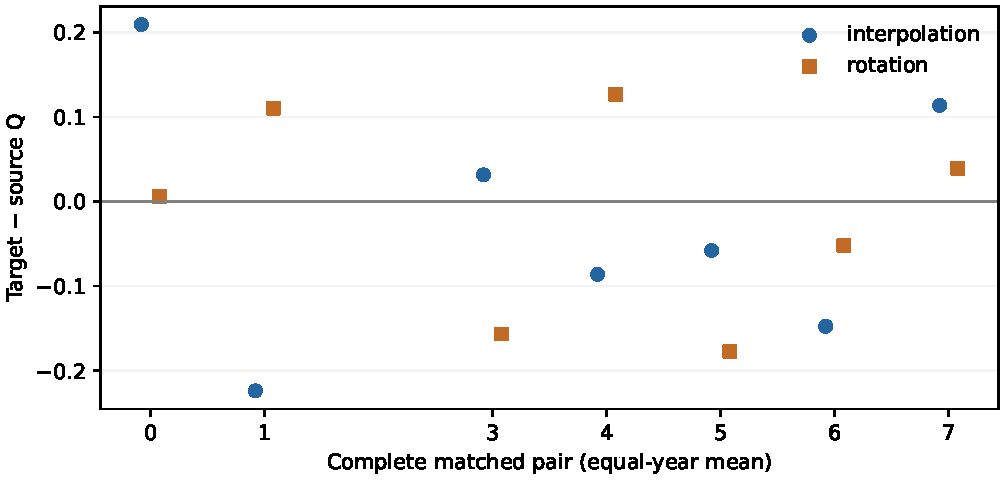
\includegraphics[width=\columnwidth]{primary_complete_pairs.pdf}\caption{Primary setting, complete pairs only. Each point averages the two years equally within its operator. Pair 2 is excluded because it has no eligible 2026 counterpart. Operator-specific signs vary; these points are descriptive components, not separate hypothesis tests.}\label{fig:pairs}\end{figure}

Figure~\ref{fig:pairs} illustrates why aggregation needs care. Pair 0 has an interpolation contrast of $+0.209$ but a rotation contrast near $+0.006$; pair 1 has $-0.224$ and $+0.110$, respectively. This is evidence of dependence on the selected controlled operator. It is not evidence that either operator reveals true institutional causes.

\subsection{Secondary reference sensitivity}
\begin{table}[t]\centering\caption{Exploratory one-hour Shapley target-minus-source $Q$. Seven complete pairs; nominal 95\% intervals, unadjusted for multiple comparisons.}\label{tab:secondary}
\begin{tabular}{llrrr}\toprule
Model&Reference&Difference&Lower&Upper\\\midrule
Ridge&Source calendar&$-0.035$&$-0.134$&0.062\\
DLinear&Source calendar&$-0.032$&$-0.148$&0.094\\
GRU&Source calendar&$-0.019$&$-0.089$&0.053\\
Ridge&History median&$-0.084$&$-0.173$&$-0.013$\\
DLinear&History median&$-0.104$&$-0.210$&$-0.015$\\
GRU&History median&$-0.068$&$-0.146$&$-0.003$\\\bottomrule
\end{tabular}\end{table}
The source-calendar one-hour intervals include zero for all three models. Under the history-hour-median reference, the three nominal intervals fall below zero (Table~\ref{tab:secondary}). These are exploratory results, and the references explain distinct prediction contrasts. They do not justify replacing the primary hypothesis after observing results or declaring the median reference defective. Six-hour contrasts also vary: the GRU history-median estimate is positive ($+0.031$), with an interval spanning zero. The full twelve-cell table is supplied in the artifact.

\subsection{Numerical audit and score availability}
Exact Shapley efficiency residuals are at most $3.56\cdot10^{-15}$ GB. Independent enumeration of all permutations on sampled Ridge, DLinear, and GRU cases agrees with the subset formula. This confirms the implemented finite game arithmetic on the audited cases; it does not validate the scientific semantics of the reference.

\begin{table}[t]\centering\caption{IG numerical acceptance across both references and horizons, frozen arm only. Cases include source/target and neural seed replicates. Failures remain recorded.}\label{tab:ig}
\begin{tabular}{lrrr}\toprule Model&Cases&Accepted&Failed\\\midrule
Ridge&480&450&30\\
DLinear&1,440&1,335&105\\
GRU&1,440&1,365&75\\\midrule
Total&3,360&3,150&210\\\bottomrule\end{tabular}\end{table}
IG passes the fixed checks in 93.75\% of cases (Table~\ref{tab:ig}). Failures can occur even for log-space Ridge because the attributed GB function contains nonlinear transformations and a clipping boundary. We did not relax tolerances or increase the quadrature limit after evaluating targets. These failures establish numerical non-acceptance under this procedure, not theoretical invalidity of IG. Comparisons of IG rankings require common accepted cases; we avoid an all-case superiority claim from its smaller subset.

Across non-IG methods, each has 53,760 operator-score records, of which 51,944 are defined. The 1,816 non-discriminating records per method have insufficient oracle--random separation. Of 6,720 IG operator records, 6,137 are scored after numerical and denominator screening. These records are repeated model/reference/horizon/operator evaluations, not independent samples. Final paired averages additionally require complete neural seeds and timestamp-matched source and target scores. Consequently, neither 168,000 total records nor 3,360 IG checks should be presented as the inferential sample size.

\section{Discussion and Limitations}
The results support a qualified operational interpretation. Similar average forecast errors do not certify stable attribution rankings across institutions. At the same time, the primary experiment does not demonstrate a systematic transfer penalty. Reference sensitivity and numerical exclusions show why a single saliency visualization or pooled score can be misleading, while the paired analysis prevents the much larger number of queries from becoming a fictitious sample size.

Several limitations constrain the contribution. First, all institutions belong to one research-network ecosystem. Cross-ISP, mobile, industrial, encrypted-flow, or attack-detection generalization is untested. The older project's heterogeneous capture datasets are not combined into this forecasting experiment.

Second, complete-history selection excludes interrupted measurements and heavily reduces some later institution-year cells. It may favor more regular traffic regimes. With only seven complete pairs and sparse sampled origins, bootstrap coverage is uncertain; 14-day blocks cannot guarantee independence across academic schedules or annual effects. Metadata matching leaves residual confounding, and the source institutions themselves are not held-out training entities. The primary contrast is a deployment comparison, not a causal effect of institutional novelty.

Third, the two replacements are controlled stress tests rather than validated draws from a conditional traffic distribution. Their forecast response can reward model sensitivity, including undesirable sensitivity. The oracle's upper bound normalizes this response game; it is not an operational utility maximum. An independently modeled traffic replacement distribution and an external network would strengthen future validation, but they were not added after the present target inspection.

Fourth, the model and explainer families are intentionally limited. We have not benchmarked foundation forecasters, specialized temporal explainers, or latent concept methods such as TimeSAE. Seven daily groups sacrifice intra-day detail. IG uses a finite quadrature budget and a smaller fixed origin subset. The exploratory intervals are not multiplicity-corrected. No alternative setting with a stronger result is promoted to the main endpoint.

\section{Reproducibility and Conclusion}
The accompanying artifact includes the frozen protocol, analysis clarifications, membership and matching tables, source and derived data hashes, 48 selected hourly series, model checkpoints, predictions, attribution allocations, numerical failure records, and analysis scripts. The pre-fit and pre-evaluation manifests remain immutable; their historical ``unscored'' fields describe the moment of freezing. A separate completion and validation record marks outcomes as scored. This is an auditable local sequence, not a public preregistration. The original dataset remains attributable to its creators under CC BY 4.0.

Final checks verify data/model hashes, recompute all forecast metrics, re-query representative predictions and labels, validate sampled Shapley games by permutation enumeration, and independently recompute the primary point estimate. These checks protect arithmetic and provenance.

We find no conclusive systematic reduction in the prespecified attribution ranking score when transferring the frozen one-hour GRU to unseen institutions. Exploratory reference-dependent differences and a 6.25\% IG numerical rejection rate motivate explicit contrast definitions, controlled-operator reporting, and exclusion audits. The contribution is an executed reliability benchmark with bounded conclusions.

\begin{thebibliography}{99}
\bibitem{transmuse} L. Xu et al., ``TransMUSE: Transferable traffic prediction in multi-service edge networks,'' \emph{Computer Networks}, vol. 221, art. 109518, 2023, doi:10.1016/j.comnet.2022.109518.
\bibitem{aichrono} P. Fern\'andez et al., ``AIChronoLens: AI/ML explainability for time series forecasting in mobile networks,'' \emph{IEEE Trans. Mobile Computing}, 2025, doi:10.1109/TMC.2025.3554035.
\bibitem{timesae} K. Oublal, Q. Bouniot, Q. Gan, S. Cl\'emen\c{c}on, and Z. Akata, ``TimeSAE: Causal sparse decoding for faithful explanations of black-box time series models,'' ICML, 2026, arXiv:2601.09776v2.
\bibitem{cesnet26} J. Koumar, K. Hynek, K. Je\v{r}\'abek, and P. \v{S}i\v{s}ka, ``CESNET-TimeSeries26: A multi-year network traffic time series dataset for annual seasonality, concept drift, and long-term anomaly detection,'' arXiv:2610.14799, 2026.
\bibitem{dataset} J. Koumar, K. Hynek, K. Je\v{r}\'abek, and P. \v{S}i\v{s}ka, ``CESNET-TimeSeries26,'' Zenodo, 2026, doi:10.5281/zenodo.21945629. CC BY 4.0.
\bibitem{dlinear} A. Zeng, M. Chen, L. Zhang, and Q. Xu, ``Are transformers effective for time series forecasting?'' \emph{AAAI}, vol. 37, no. 9, pp. 11121--11128, 2023.
\bibitem{gru} K. Cho et al., ``Learning phrase representations using RNN encoder--decoder for statistical machine translation,'' \emph{EMNLP}, 2014, arXiv:1406.1078.
\bibitem{comparison} J. Koumar, T. Smole\v{n}, K. Je\v{r}\'abek, and T. \v{C}ejka, ``Comparative analysis of deep learning models for real-world ISP network traffic forecasting,'' arXiv:2503.17410, 2025.
\bibitem{aggregated} A. Knapi\'nska and K. Walkowiak, ``Explaining aggregated network traffic predictors,'' \emph{IFIP Networking}, 2025. \url{https://opendl.ifip-tc6.org/db/conf/networking/networking2025/1571141805.pdf}.
\bibitem{deexp} S. Moghadas Gholian et al., ``DeExp: Revealing model vulnerabilities for spatio-temporal mobile traffic forecasting with explainable AI,'' \emph{IEEE Trans. Mobile Computing}, 2025. \url{https://hdl.handle.net/20.500.12761/1889}.
\bibitem{ig} M. Sundararajan, A. Taly, and Q. Yan, ``Axiomatic attribution for deep networks,'' \emph{ICML}, PMLR 70, pp. 3319--3328, 2017.
\bibitem{shap} S. M. Lundberg and S.-I. Lee, ``A unified approach to interpreting model predictions,'' \emph{NeurIPS}, vol. 30, 2017.
\bibitem{manyshap} M. Sundararajan and A. Najmi, ``The many Shapley values for model explanation,'' \emph{ICML}, PMLR 119, pp. 9269--9278, 2020.
\bibitem{baselines} P. Sturmfels, S. Lundberg, and S.-I. Lee, ``Visualizing the impact of feature attribution baselines,'' \emph{Distill}, 2020, doi:10.23915/distill.00022.
\bibitem{sanity} J. Adebayo et al., ``Sanity checks for saliency maps,'' \emph{NeurIPS}, vol. 31, 2018.
\bibitem{perturb} J. Enguehard, ``Learning perturbations to explain time series predictions,'' \emph{ICML}, PMLR 202, pp. 9329--9342, 2023.
\bibitem{interprettime} H. Turb\'e et al., ``Evaluation of post-hoc interpretability methods in time-series classification,'' \emph{Nature Machine Intelligence}, 2023, doi:10.1038/s42256-023-00620-w.
\bibitem{timing} H. Jang, C. Kim, and E. Yang, ``TIMING: Temporality-aware integrated gradients for time series explanation,'' \emph{ICML}, PMLR 267, pp. 26877--26895, 2025.
\end{thebibliography}
\end{document}
